\chapter{Introduction}

Today, technology is used for all kind of purposes, and it has become an important part of people's everyday life. Different kinds of technologies meet a wide range of needs, all from entertainment and socialisation, to education and health. One focus that has got great attention the last years is how to use video games with motion sensor technology to engage people in exercise and physical activity \cite{exergamesforelderly}, \cite{gerling1}, \cite{garcia2012exergames}. These games are called exercise games, or exergames, because they require body movements to play. There have been done a lot of research on different motion sensor technologies used for exercise and it has shown positive effect when it comes to improving peoples health. 

Due to "baby boomers" and the fact that people are living longer, the world's population now consist of a great share of older people \cite{dickinson2007methods}. As a part of growing older, elderly often meet disabilities like physical and psychological decline. Due to reduced balance function and physical strength, one serious problem for elderly people is the risk of falling. Fall is the leading cause of injuries in older people, and can often have serious consequences \cite{otago}. These problems, together with the world's ageing population, lead to both strategical and economical challenges for the government when it comes to providing health care services to everyone that need it. This clearly shows that new initiatives have to be taken to identify how to prevent falls, and keep the older population healthy. However, engaging the elderly population in physical activity can be challenging, and it is shown that a great share of elderly do not exercise enough \cite{statistikknorge12}. The introduction of an exergame can meet this problem. This can serve as a more fun and entertaining alternative than regular exercise.  

The use of exergames for health related purposes is supported by the new reform "Samhandlingsreformen" in Norway, were one focus is to use welfare technology in the health sector where possible \cite{welfare}. However, many older people are unfamiliar with technology, and especially with video games. In addition, existing commercial exergames are aimed towards a younger user group, and are therefore not suitable for elderly \cite{exergamesforelderly}. A first step to make the older population accept the use of video games for health related purposes, would be to develop a game aimed especially for their needs and interest, where their physical and psychological declines are taken into consideration. 

This thesis is built upon our project assignment \emph{Business Opportunities and Economics for an Exercise Game in the Health Sector} \cite{project}, where we developed a business model for an exergame, with the physiotherapy service as the customer. In this thesis we will focus on the end users of this game, which are elderly people. Our contribution in this thesis will be to explore and identify the users' needs and wants, gather sufficient knowledge and information about system design, and from this create a concept\footnote{We have choose use the term \emph{concept} which means \emph{an idea, or a general notion} http://dictionary.reference.com/browse/concept} for an exergame appropriate for the older user group.

\section{Objectives}
\label{sec:researchq} Exergames have shown promise in health related purposes like for exercise and rehabilitation. However, previous research suggest that commercial exergames are not suitable for elderly, as they are not specially aimed and developed for this user group \cite{exergamesforelderly} \cite{gerling2} \cite{bruin} \cite{project}. 

We will study how elderly interact with commercial Xbox Kinect games to see what do and do not work, and to validate previous findings. With this we will answer research question 1 and 2: 

\emph{RQ1: Are existing commercial Xbox Kinect games suitable for exercising purpose for elderly people?} 

\emph{RQ2: What are the design challenges when developing an exergame for elderly people, and what aspects need to be considered in this game?}

Based on the answers to research questions 1 and 2, and theory and knowledge about video game development, usability and system design, we will answer research question 3:

\emph{RQ3: What would be suitable system requirements, and appropriate design, for an exergame for elderly people?}

\section{Contribution}

Our contribution in this thesis is the development of system requirements and a concept for an exergame for elderly people. Some aspects from our previous project \cite{project} have been used as motivation for this thesis. A brief summary of this will be provided in Chapter \ref{chap:background}. To be able to understand the users, we have looked into challenges and motivating factors when it comes to engaging elderly to perform physical activity. This will be presented in Chapter \ref{chap:olderexercise}. For the reader to get an insight into what exergames are, we provide in Chapter \ref{chap:exergames} a brief overview of this. As we are making an exergame concept, we have studied important aspects related to game development for the older user, and summarised a set of guidelines that should be followed when developing for this group. This can be found in Chapter \ref{chap:exforseniors}. Understanding of the different elements included in a video game, as well as general system design, is needed to develop the exergame. We provide an introduction to these topics in Chapter \ref{chap:vg} and \ref{chap:generalsystemdesign}, respectively. In accordance with the importance of user involvement, we have conducted two workshops where we have engaged users in the development of the exergame. Informants were recruited by holding a presentation for "Seniornett", an organisation working with teaching the older population technology. This will be described in Section \ref{sec:recruitment}. Workshop 1 was conducted to observe and understand how a group of elderly people interact with commercial Xbox Kinect games. In this workshop, methods like questionnaire, participatory observation and focus group interviews were used. These methods are described in Chapter \ref{chap:metode}. We observed the informants play three games chosen by us, and followed with a focus group interview. A description of the execution, and findings from workshop 1, will be presented in Section \ref{sec:ws1} and in Chapter \ref{chap:findW1}, respectively. The main focus for this thesis has been to specify system requirements and create design for a concept for an exergame for elderly people. This work has been based upon information gathered from theory, previous studies and findings from workshop 1. The design was presented by making prototypes. The exergame concept is the most important contribution in this thesis, and will be presented in Chapter \ref{chap:concept}. The concept was presented in a second workshop, to be evaluated by the users. The execution of, and findings from, workshop 2 are presented in Section \ref{sec:ws2} and Chapter \ref{chap:findW2}. In our discussion, provided in Chapter \ref{chap:discussion}, we provide a detailed description of future work for an exergame for elderly, based upon findings from workshop 2. This thesis provides general guidelines for how to design an exergame for elderly, and can be used in the continuation of our exergame concept, or in the development of a new exergame. The main findings in this thesis, together with the design proposal, have been presented in a workshop with the EU-project FARSEEING \footnote{FARSEEING is a collaborative European Commission funded research project, which are working on promoting healthy, independent living for elderly people with the use of technology. See http://farseeingresearch.eu/ for more information.}.

\section{Work Process} 
Figure \ref{fig:workflow} presents the work process for the present thesis.   
\begin{figure} [H]
\centering
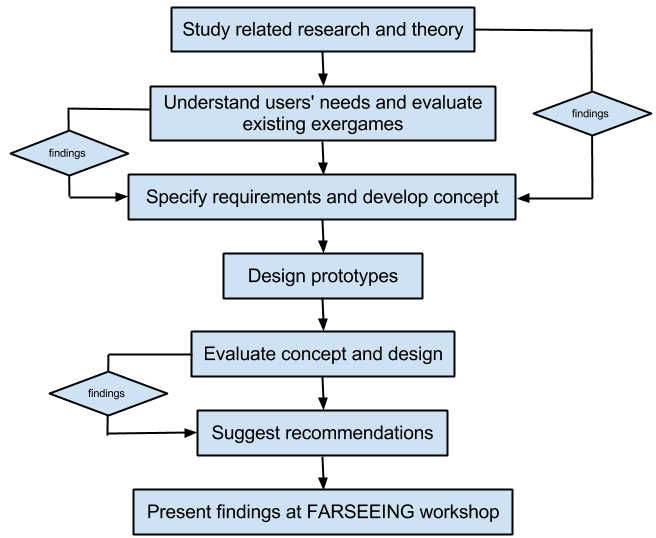
\includegraphics[scale=0.7]{Workflow.png}
\caption[Work process]{Work process}
\label{fig:workflow}
\end{figure}

\section{Scope and Limitations}
One important limitation of this thesis is the sample of informants in our workshops. Elderly cannot be seen as one common group of people. They are people with different interests and needs. In this thesis, we only included one small group of elderly. Due to time limits before the first workshop, which was critical for our further work, we only recruited informants from the organisation "Seniornett". We did not have the time to look into other arenas for recruiting. The informants had never played video games before, which made it challenging to include them in the development process of the exergame concept. Gathering a group of elderly, and observing them while they played different Xbox Kinect games, is not observing a natural setting. This made it difficult to fit this study into defined research methodologies. The last limitation concerns the choice of how we presented our design. We used prototypes, but limited them to not involve any interaction, even though they represent scenarios for a highly interactive game.  


\section{Outline}
The report is structured in the following way:

\begin{itemize}
\item In \textbf{Chapter 2} the main background and motivation for this master thesis will be presented.
\item To make a video game aimed for exercising, there is a need to understand what actually motivated elderly to exercise in general. This will be provided in \textbf{Chapter 3}. In addition, we will briefly discuss how elderly should exercise.
\item In \textbf{Chapter 4} we will describe what video games, and in particular exergames, are. We will also present the exergame technology we have made an exergame concept for, namely Microsoft Kinect.
\item Elderly people are a group with diversity, and have some typical characteristics. A lot of research on how to make appropriate exergames for elderly people, where these characteristics are been taken into account, have been conducted. In \textbf{Chapter 5} we summarise interesting research and provide a list of typical characteristics of elderly, as well as guidelines for how exergames and user-interfaces should be made for this group.  
\item In \textbf{Chapter 6} we present video game design in general. This is to make it easier to structure our exergame proposal, and to include important elements that a video game should consist of.
\item It is also important to understand how to design systems in general. In \textbf{Chapter 7} we will discuss the four pillars of design, system requirements and the importance of usability. At last, we will present a model that can be used for usability evaluation of games or as guidelines in an early development phase. 
\item It is important to involve the user in the development process of a system. This can be done with several methods, which we will discuss in \textbf{Chapter 8}. This includes; experimental simulation, participatory observation, focus group interview, questionnaire and video and audio recording. At last in this chapter, a thorough description on how we have worked, and how we have used the different methods will be described.
\item In \textbf{Chapter 9} the findings from workshop 1 will be presented.
\item Based on the theory discussed in the previous chapters together with the findings from workshop 1, we will present the functional and interface requirements and the exergame concept. This can be found in \textbf{Chapter 10}. As a part of this, prototypes of some scenarios in the game will be shown.
\item The exergame was evaluated by a group of elderly in a second workshop. In \textbf{Chapter 11} the findings from workshop 2 will be presented.
\item In \textbf{Chapter 12} our findings and result will be discussed and we will provide recommendations for future work on our exergame, based on the feedback gotten from workshop 1. The quality of the research will also be discussed.
\item Finally, in \textbf{Chapter 13}, we provide a conclusion on the work done and we suggest future work.

\end{itemize}
